\documentclass[11pt, a4paper]{article}
\usepackage[utf8]{inputenc}
\usepackage{graphicx}
\usepackage{graphics}
\usepackage{amsmath}
 \usepackage{cite}
%\usepackage[style=authoryear]{biblatex}
%\addbibresource{ref_list.bib}
\usepackage{rotating}
\usepackage[margin=1.12in]{geometry}
\graphicspath{{images/}}
 \linespread{1.50}
\usepackage{hyperref}
\usepackage{amsmath}
\usepackage{titlesec}
\usepackage{caption}
\setcounter{secnumdepth}{4}

\title{Msc Data Science Project Proposal, Department of Computer Science and Information Systems, Birkbeck College, University of London\\ \textbf{The Applicability of Machine Learning Methods For Currency Trading} }
\author{Edward Gill } %\thanks{adding thanks}
\date{ $15^{th}$ April 2019}

\begin{document}
\maketitle

\begin{abstract}
To be decided closer to the completion date
\end{abstract}
Date: 16 April 2019\newline
Supervisor: Dr. George Magoulas \newline
M.Sc. Data Science project proposal, Department of Computer Science and Information Systems, Birkbeck College, University of London, 2019
This proposal is substantially the result of my own work, expressed in my own words, except where explicitly indicated in the text. I give my permission for it to be submitted to the JISC Plagiarism Detection Service.
The proposal may be freely copied and distributed provided the source is explicitly acknowledged.


\clearpage
\tableofcontents

\clearpage


\section{Introduction}

The velocity of technological change that society has encountered since the turn of the millennium is striking, the world has embarked on a technological revolution which has brought the availability of immense processing power to the masses. Computational power so large that government sponsored computer science programs of the early nighties could only dream of, in fact, the processing power of most smartphones are larger than the supercomputers of yesteryear \cite{supercomp}.
\newline Moore's Law, the well known law which states that the number of transistors in a dense integrated circuit doubles about every two years, has held for over fifty years \cite{MacK2011}. 

\par
The rise in computing power has opened a veritable Pandora's box of highly complex and computationally intensive models which can now be applied to any data set, whether appropriate or not. While machine learning models have led to rapid and impressive use cases across a host of different fields of research, this paper will focus on one oft researched area, global financial markets and specifically currency markets.
The allure of applying machine learning methods to finance is well entrenched, where researchers dream of finding the holy grail of a repeatable pattern within the data which leads to guarantees of consistent alpha generation (returns unexplained by conventional market beta factors \cite{Rebonato2017}).
\par 
A cursory search of Google, another revolution of big data processing and clustering algorithms, uncovers a plethora of academic papers which profess of having found patterns in the data that could only have been uncovered by complex models with non-linear capabilities. While big data and machine learning models can and do give fantastic results in the area of the biological sciences or as recommender systems for movies or advertisements, applying these same methods to financial markets is a different and more challenging task due to the underlying unpredictability of financial markets.\par

This proposal will firstly outline prior research undertaken alongside some of the more common pitfalls that can impact model performance and model generalisation. The rest of this proposal dives into the data to be used, model building framework , main pitfalls which make applying complex algorithms in finance susceptible to out of sample failure \cite{LopezdePrado2018} and also a brief analysis of the potential machine learning methods to be used.
\par

\section{Background}

The task of uncovering repeatable patterns in financial data remains incredibly precarious, financial markets are non-stationary, exhibit leptokurtic (fat tailed) distributions and can shift regimes at highly unpredictable speeds. Figure \ref{fig:eurvol} shows the 1 year rolling volatility of EURUSD (with daily snapshots created at 8am and 4pm). We can clearly see how volatility remains non constant over time and that even the time of day used to calculate the volatility can allow large deviations to in volatility to persist.
\begin{figure}[h]
    \centering
% below is where you put the acutal image name in the directory
  \caption{EURUSD Rolling Annualised Volatility Since 2002}

    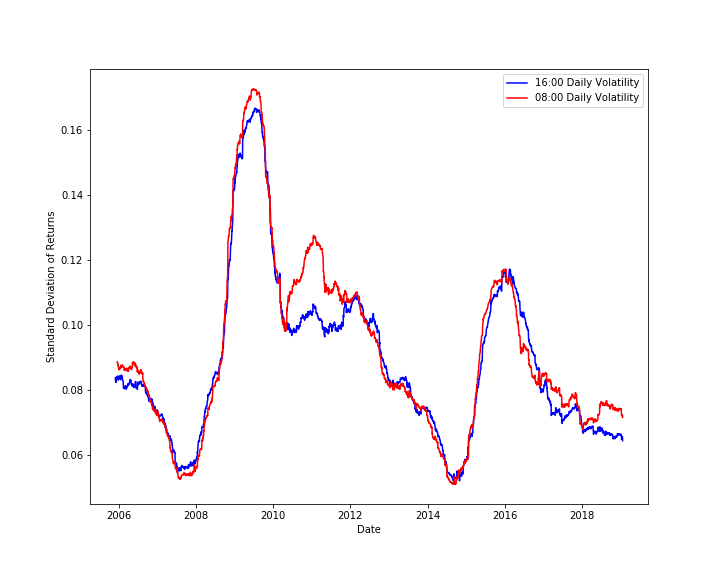
\includegraphics[width=0.75\textwidth]{EURUSDRollingVol}
   %  below is only a naming convention, above is the real deal
    \label{fig:eurvol}
\caption*{Source: EURUSD FX Rate, Kaggle Database}
\end{figure}
\newline
Much has been written on the complexity of financial markets and how researchers must overcome such dynamic systems \cite{Lebaron1994}. While the explosion of increased computational power aided the application of machine learning in very useful tasks such as speech recognition and image processing, the applicability of these methods in finance are, on the face of it at least, questionable \cite{Bailey2013}. 
\par
In the era of big data, financial markets are one domain which has some of the smallest datasets available, as one important factor is in short supply, time. Financial timeseries have relatively little history when compared to other fields of study. Most accurate data capture goes back to the early nineties and unless the domain is high frequency tick data, then there generally is sparse data to test with when compared to some non-financial data sets such as movie recommendation algorithms, which have many millions of users each with their own individual movie met data attributes \cite{Portugal2018}. 

\section{Aims and Objectives}
The main aim of the project is to understand how machine learning methods can be applied to currency forecasting and the classification of macroeconomic regimes in which a particular model (or combination of models) may perform best.
\par The project will try to outline best practices when applying machine learning techniques to currency trading, this may take the form of an outright prediction model or a set of models which also forecast shifts in market regimes. This will allow us to combine information from various sources to provide the highest probability of out of sample trading success.

The main objectives in order to achieve the stated aim of the project are shown below.

\subsubsection{Data Retrieval, Cleaning and Standardisation}
\begin{itemize}
\item One of the most important aspects of a trading model is to ensure that the underlying data is of high quality and doesn't contain erroneous values. The proposed model will use hourly spot exchange rates for G10 currencies \footnote{Hourly FX Spot Data Provided by Citi Foreign Exchange}, various economic data from the Federal Reserve Economic Database (FRED), the International Monetary Fund (IMF) and the Organisation for Economic Cooperation and Development (OECD) will be used to try to uncover exploitable patterns in the data. 
\item This data will also need to be cleaned and mapped to correct date scales so that the model only uses data available at the time of trade signal generation. The raw data itself will need to be standardised to allow the model to understand the true relationships between the features and the output.
\end{itemize}
 \subsubsection{Feature Extraction}
	\begin{itemize}
	\item Feature extraction for financial time series prediction is a very challenging task and given the inherent noise in the data,including features which have an intuitive justification for predicting future prices is important \cite{Arnott2018}. Feature selection driven by mining the training set greatly increases the risk of overfitting and should be avoid when working with financial times series. 
	\end{itemize}
 \subsubsection{Model Training and Architecture Selection}
	\begin{itemize}
	\item The project itself will test the efficacy of a range of algorithms in trying to predict currency movements, this project will also make use of non price data in order to assist the model in understanding potential regime changes in the trading environment. 
	\end{itemize}
 \subsubsection{Model Validation and Strategy Back testing}
	\begin{itemize}
	\item Once a model architecture has been selected, it is important to understand not only classification rates but also how the model would perform in a live market setting. This can be approximated by creating a back testing framework which depicts the models trading performance and also includes the impact of transaction costs.
	\end{itemize}
\subsubsection{Testing on Fully Withheld Data}
	\begin{itemize}
	\item While the test data allows us to understand how the model performs, there will also be an opportunity to analyse how the selected model will work on new unseen data which would provide a useful guide to model generalisation in the future.
	\end{itemize}

\section{Pitfalls of Machine Learning in Trading}
The problem to overcome in applying ML to trading is the level of signal to noise in the data. To try to differentiate the problems ML practitioners face in the financial domain vs others, lets looks at an example. Take the case of image processing, if a neural network is fed a matrix of pixels which form the image of cats and dogs, and the neural network trains the model based on the historical patterns it observes. The well trained neural network will no doubt be able to identify cats and dogs with high classification rates, however, if we provide an image of a rhino, the model likely classifies the rhino as a large dog due to the historical patterns that have been learned. \newline Similarly with the Alpha Go project \cite{Silver2016} at the company Deep Mind, the developers created an excellent model which would calculate all possible combinations of moves to find the most optimal route to victory. This model convincingly beat the worlds best human Go players.
\par
That extremely well built model is beholden to the past patterns it has learned over millions of iterations playing within the well defined rules of the game of Go. In finance, which one could assume is somewhat akin to playing the ancient game of Go (or more closely related would possibly be poker) you can learn all the historical patterns and probabilities surrounding the asset you are trading. This model will likely work very well even in the testing period. However, in finance the rules can change rapidly, causing structural breaks to occur in past relationships. Alpha Go does not need to worry about the impact of a 280 character tweet from Donald Trump entirely changing the rules of the game.\newline 
For example, in the run up to the 2016 US presidential election, equity markets would sell off due to increases in Donald Trump's odds of winning the presidency. The market was horrified to see a president who openly criticized western allies, spoke of protectionism and of building walls against major trading partners. 
\begin{figure}[h]
    \centering
% below is where you put the acutal image name in the directory
 	\caption{US Equity Market Performance During Election Week}
    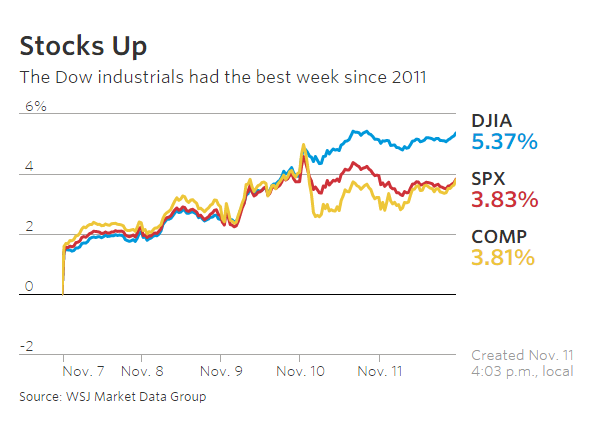
\includegraphics[width=0.65\textwidth]{ElectionDay}
 %  below is only a naming convention, above is the real deal
    \label{fig:election}
	\caption*{Source: Wall Street Journal, Nov 2016}
\end{figure}

However, post his initial speech (which was much less controversial and business friendly) markets fully reversed any losses and ended 5\% higher (figure \ref{fig:election}). Thus even models that had predicted a Trump win (and subsequent market crash) and positioned as such based on the historical correlations in the lead up to election day would have incurred severe losses. Currency markets were also impacted , with EURUSD rising nearly 3\% as the election result was announced, before subsequently falling by an even larger amount after Trumps conciliatory speech \ref{fig:EURElection}. 
\begin{figure}[h]
    \centering
% below is where you put the acutal image name in the directory
	\caption{EURUSD Price Action During Announcement of the 2016 US Presidential Election}
    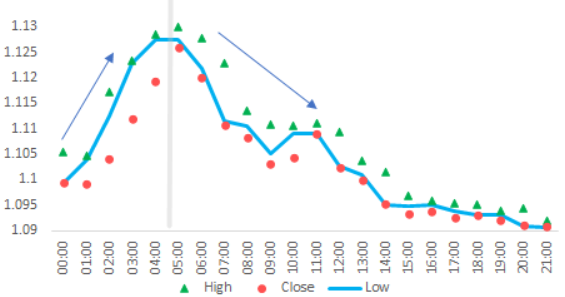
\includegraphics[width=0.75\textwidth]{EURUSDElection}
 %  below is only a naming convention, above is the real deal
    \label{fig:EURElection}
	\caption*{EURUSD FX Rate, Kaggle Database}
\end{figure}
\par Correlations and patterns in markets can be extremely fickle complex and dynamic nature \cite{Camargo2013}. Why is this so one may ask, well part of the issue lies in the efficiency of informational flow across markets currently, barriers to entry are much smaller and there has likely been a compression in the informational edge that smart money investors (such as hedge funds) previously have had \cite{hedgefundRets}. The market price itself is a reflection of all these moving parts and thus even if a robust pattern has been found, it is likely to be arbitraged as more market actors step in to trade away any mis-pricing \cite{Bartram2019}. 
\par
One issue that is particularly pertinent in the financial domain is the issue of data dimensionality and the underlying size of each individual data set, even if there was fifty years of daily financial data, this is less than 20,000 data observations\footnote{Assuming a 252 trading day calendar}, thus while in other fields of research there may be millions of data points for categorisation and training, this is not the case for finance. This means that one must think carefully before adding features to the model. There are thousands of potential predictors of a financial asset (in fact Chatzis et al. used 180 predictors when trying to forecast financial market crisis events \cite{Chatzis2018} ), and this means that due to the number of possible variations, the probability of finding a strategy by luck remains high, Arnott et al. provide an example of a trading strategy which would have passed even the most stringent evaluation methods in both training, validation and testing phases which actually turned out to have been created using a ranking of stocks based on alphabetical ordering \cite{Arnott2018}.

\subsection{Heteroskedasticity in Financial Markets}

Complex systems that continuously evolve make applying ML techniques in a way that results in a robust model very difficult \cite{Arnott2018}. Financial markets have been shown to exhibit heteroskedasticity in their returns \cite{Corhay1996} and as such creating a robust systematic trading strategy relies on more than just a simple data input/signal output type of architecture. \newline In trading systems, classification of regimes and subsequent buy or sell signals must also be compared vs the expected value of the that trade. A model with an 80\% classification success rate will under perform if it mis-classifies the the 20\% of samples which result in large moves in the asset. The corollary of that is by only targeting classification of outliers you reduce your sample set and thereby reduce the statistical validity of the results. There is rarely a free lunch in financial markets and as such there will be no free lunch in using machine learning methods to predict financial times series. 
For example figure \ref{fig:beststockdays}, shows that if an investor were to miss out on the best 25 days of the Standard and Poors 500 companies equity index (S\&P 500) over the last fifty years, the reduction in returns would have been very severe \cite{bestdays}. Given that 25 trading days represents only 0.005\% of the total trading days , returns are significantly impacted. This shows the importance of being correctly positioned for outlier events and also the fact that one model can be severely impacted by one off or black swan type events \cite{Taleb2007}.
 
\begin{figure}[h]
    \centering
% below is where you put the acutal image name in the directory
	\caption{Growth of \$100 Invested Since 1975}
    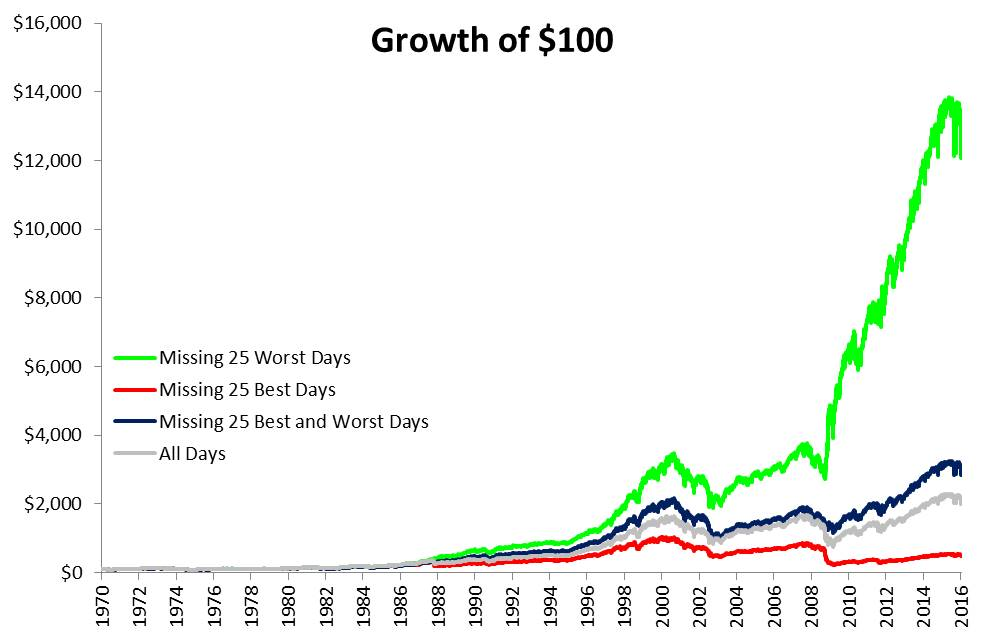
\includegraphics[width=0.65\textwidth]{beststockdays}    
 %  below is only a naming convention, above is the real deal
    \label{fig:beststockdays}
	\caption*{Source: Market Watch\cite{bestdays}}
\end{figure}
Previous research has centered on price based data possibly as it is easily available and also because it is one dataset that is likely to have higher frequency data available (\cite{Huang2005},\cite{Shen2012},\cite{Wang2014}). 

\begin{figure}[h]
    \centering
% below is where you put the acutal image name in the directory
	\caption{Distribution of Currency Returns Shifts According to The Market Regime}
     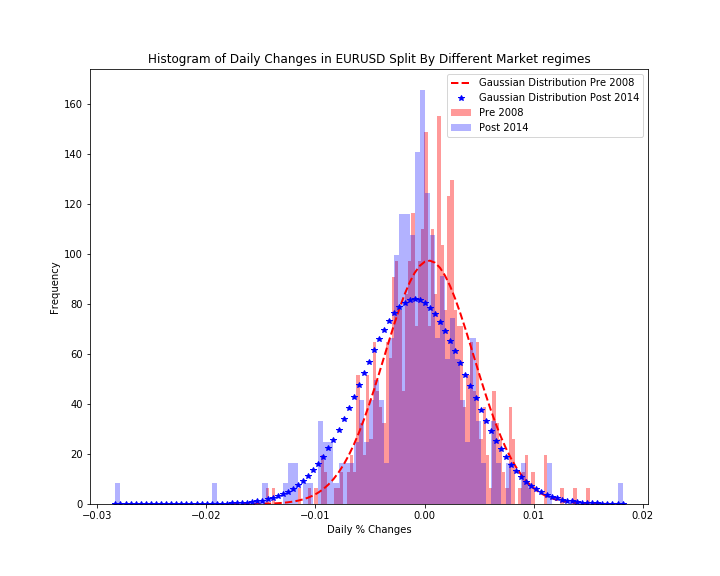
\includegraphics[width=0.65\textwidth]{Regimehist}
 %  below is only a naming convention, above is the real deal
    \label{fig:Regimehist}
\caption*{Source: EURUSD FX Rate, Kaggle Database}
\end{figure}
In fact, even when analysing the daily changes in EURUSD , we can see that the distribution of future returns can shift quickly, and the regime a model has learned in can end up shifting so that the model's future predictions under perform. For example, figure \ref{fig:Regimehist} splits daily distribution of EURUSD percentage returns by two different regimes, one in 2008 vs a second regime in 2014, each market regime results in a shift in the distribution of the currency and thus when training a model, one must be cognizant of the impact the wider market regime can have on a models performance.

\clearpage
\section{Building Blocks of Currency Trading Strategies}
One area which seems under researched (from the research performed), is to use lower frequency economic data to assist in a model's prediction accuracy. While price based metrics offer the easiest route to higher frequency data, they also lack the ability to capture the fundamental economic factors that can drive currency direction \cite{medium}. 

\subsection{Drivers of Currency Markets}

Firstly, before we analyze feature selection methods, it is also important to try to understand what consists of a good trading signal, whether discretionary or systematic in its generation. Below we showcase factors that can impact currency specific direction.
\subsubsection{Economic Fundamentals}
One of the most important factors that sets the broad direction of a currency is the relative economic performance between two countries.
Dahlquist et al. show that measuring relative economic momentum between different countries has the ability to forecast currency direction over medium term horizons \cite{Dahlquist2015}. That paper showed statistically significant results that economic fundamentals have an important role in relative capital flows and subsequent currency direction.
\subsubsection{Price momentum}
Price momentum here refers to the historical trend in the currency,  research does suggest there exists  exploitable momentum within the currency space \cite{Moskowitz2012}. The reasoning for the existence of momentum in currencies is likely due to decision delays amongst different investor segments who build up positions in currencies over time. Auto-correlation in currencies may also exist as information is priced slowly over time (such as economic data) and thus as more economic data is published, this adds further confirmation to a trading signal and thus conviction and trade size increases.
\subsubsection{Investor Positioning}
Currency positioning relates to the current magnitude of investor holdings of a currency. Positioning and currency flows can have informational value that impacts a model's performance \cite{Menkhoff2012}. For instance, if the finalised model triggered a buy recommendation on a currency, but if the wider market had already built up a sizable long position in that currency, then the likelihood of further buyers coming in to drive the price higher is diminished.
\subsubsection{Currency Valuation}
Uncovering the true fundamental fair value of a currency has been the focus of international academic research for many years \cite{Rogoff1996}, and it remains an elusive and rather ambiguous task as currency drivers can undergo structural shifts. Purchasing Power Parity currency levels  , which rely on the Bassala Samuelson effect and the law of one price \cite{Hassan2016} are one method of trying to anchor the value of a currency to one fundamental price level. While currencies can deviate from fair value, there is some evidence that developed market\footnote{Developed Market Currencies consist of USD, EUR, JPY, CHF, GBP, AUD, NZD, NOK , SEK, CAD} currencies tend to mean revert in the long term \cite{CaZorzi2016}.


\subsection{Using a Multi Factor Model For Currency Prediction}


While the above drivers of currency markets are not exhaustive, it can provide a frame work for constructing a systematic trading strategy. Currency drivers can shift over the short and medium term and while this can all be partially captured by price action, it is also prudent to try to understand the dynamics of other potenial drivers as discussed in the previous section. \newline
Therein lies the main problem when combining machine learning and finance, that other areas such as the biological or physical sciences do not encounter, is that at the core of each price, are human or human created trading algorithms which have collectively decided on a price level at which to transact. \newline Every price of a trade in financial markets consist of the dreams, fears and greed of human emotion. Not only this, but market investors are influenced by past patterns and incorporate new information (including newly published research) into future decisions, thus altering the environment in which the historical pattern has been learned. Bartram at al. provide evidence that anomaly (excess) profits published in research papers tend to decay substantially in the period after publication, which suggests any new findings are arbitraged away \footnote{Of course a more sinister reason could be model overfitting on historical data} quickly as the new information is incorporated into the market\cite{Bartram2019}. 

While early academic research espoused the efficient market hypothesis, there are certain times where the market is not fully rational \cite{Dome2008}. Thus opportunities do exist, but finding repeatable opportunities requires more than just analysing price patterns in data. Given the randomness of markets, even poor strategies can perform well for long periods of times due to sheer luck. This creates new challenges for practitioners of machine learning in finance, in fact, new research has also started to focus on protocols and best practices around data mining in finance \cite{Arnott2018}.
\subsection{The Myth of Machine Learning in Finance?}
Given the inherent challenges faced when developing systematic trading strategies, one may wonder if creating a strategy based on machine learning methods is a fruitless endeavor.
\newline Due to the unique issues related to applying machine learning in the financial domain, this paper proposes to test various models with the goal of finding a robust methodology for extracting features which also have the ability to generalise into the future. Once the results and performance of each model has been obtained, it is then vital to compare and contrast how each model performs both in the training and validation phases. \newline To ensure we can test the selected model fully  on new data, the last one year of test data will be truncated from the data until all validation and testing phases have been completed, this allows us to see how the finalised model would perform on fully unseen data even after initial testing and calibration phases across all the models selected.

\section{Machine Learning Model Overview}
 Below we provide a brief overview of various models we will test in our analysis and that have been utilised in previous research.

\subsection{Artificial Neural Networks}
Artificial Neural Networks (ANN) were conceptually first written about in the early 1940s \cite{Widrow1990} when neurophysiologist Warren McCulloch and mathematician Walter Pitts wrote a paper on the theoretical functioning of neurons, Donal Webb then expanded on this in his paper "The Organization of Behavior" while the first computerised neural networks were developed by IBM in models called "ADALINE" and "MADALINE" \cite{Widrow1990} . At their core, ANNs are a series of large matrix multiplications where weights and biases , which represent the strength of connections between nodes, are optimized to provide the best approximation to the desired output. The popularity of ANNs have grown as enhanced computational power led to the lowering of barriers to entry in the field. One of the more popular networks used in practice is the mutlilayer perceptron, initially introduced by Frank Rosenblatt in 1958 \cite{Rosenblatt1958}. A perceptron is the simplest form of a layered network and consists of a single neuron with an adjustable weight. The simplest form of the perceptron can divide the hyperplane into a 2-dimensional space which is then used to classify the given inputs. The hyper plane is defined by the linearly separable function below.

\begin{align}
\sum^{n}_{i = 1} x_{i}w_{i} - \theta = 0  
\end{align}

Multi Layered Perceptrons (MLP) can be defined as 
\begin{align}
NeuralNet^{l}_{j} =  \sum^{N_{l}}_{i = 1}w^{l-1}_{ij} y^{l-1}_{i}  
\end{align}
where $NeuralNet^{l}_{j}$ is the $l$th layer of the $j$th neuron which gives us the weighted sum of its inputs. The weights of the connections to the next layer $l=1$ are used to calculate the weighted sum of inputs for the subsequent layer in the network.  \begin{align}
Y^{l}_{j} =  ActivationFunction(NeuralNet^{l}_{j})  
\end{align} 
This weighted sum of inputs is then passed through to an activation function which maps the output of the hidden layer to a space defined by the activation function, in this step we can introduce non linearity into the model itself by using a non linear activation function such as the sigmoid function described below.
\begin{align}
y =  \frac{1}{1+e^{-x} }
\end{align} 
This maps any series of values onto a plain of [-1,1] and the output depends on the values produced by the node which feeds the activation function. \par While there are a vast array of model training techniques , one method to train an ANN is to use backpropagation, where updates to the networks weights are fed backwards through each layer. Each model has an error function which is used to grade performance, which could be the the squared difference between the models output and the desired output (mean squared error).  \newline The universal approximation theorem \cite{Kurkova1992} of the MLP model in neural networks states that ANNs can approximate any function and thus in theory, should be able to identify any patterns within the data that another method would also identify. \newline The temptation to introduce multiple layers with thousands of connections in order to find a solution is ever present, however (and especially in the realm of finance) this increases the risk of over-fitting or selecting a model based on sheer luck, which fails when tested on live unseen data. 
\subsubsection{Background Research}
ANNs have been used extensively in academic financial journals, Czekalski et al. made use of feedforward multilayer perceptrons to prediction the direction of the EURUSD currency rate \cite{Czekalski2015}, while Wang et al. applied probabilistic neural networks and  Least Square Support Vector Machine models to assist in the prediction of Chinese equities \cite{Wang2014} . Literature on using ANNs to forecast currencies has a twenty year history as even at turn of the millennium Joarder et al.  tested three separate ANN based forecasting models using standard backpropagation, scaled conjugate gradient and backpropagation with Baysian regularization to predict movements in various Australian dollar currency crosses \cite{Joarder2013}. Gunduz et al. tested a variety of ANN models and Support Vector Machines (SVM) to try to predict the price of equities traded on the Istanbul Stock Exchange, they uncovered model classification accuracy consistently around 70\% on test data \cite{Gunduz2017} . \newline The majority of research cited make use of various technical indicators which are derived directly from the price series, for example,Gunduz et al. make use of ten price based technical indicators to uncover patterns within Turkish equities \cite{Gunduz2017}. While on average most prior research suggested above 70\% classification rates were attainable on average. In contrast to this, there has also been some research to suggest that ANNs often show inconsistent performance on noisy data (\cite{Kim2003},\cite{Kumar2006},\cite{Kim2000}), which highlights the challenges in applying complex models as the risk of overfitting the data remains an ever present threat. 

\subsection{Support Vector Machines}
One model which prior research suggests is useful for uncovering repeatable patterns in financial data are Support Vector Machines (SVM) and Support Vector Regression (SVR). SVMs were initially introduced by Cortes and Vapniks \cite{Cortes1995} which led to the development of non-linear models which provide binary classifications of target vectors while SVRs output real-valued predictions. In similar fashion to an ANN, the SVM tries to classify an n-dimensional feature vector according to where that data lies on an n-dimensional space.
\newline The model makes use of the kernel trick \cite{kerneltrick} to transform the original data into a higher dimensional space such that we can then uncover a separable hyperplane. The function updates the parameters of the kernel function such that it can more accurately separate and classify the data points. The error correction model in the case of a SVM is a maximisation problem where the model tries to maximise the distance between all the separating hyper planes (maximal margin classifier) it has constructed.  The maximisation problem can take the form of the following

\begin{align}
Maximise  \sum^{N}_{i = 1}w_{i} - \sum^{N}_{i = 1} \sum^{N}_{j = 1}w_{i}w_{j}*y_{i}y_{j}*K(x_{i},x_{j}) 
\end{align}

where $w_{i}$ denotes the coefficients of the $i^{th}$ observation $(i = 1,2,...,N)$, $y_{i}$ is the output of observation $i$ and $x_{i}, x_{j}$ are vectors which undergo dimensional transformation using the selected kernel.
\subsubsection{Background Research}
 Kara et al. utilised SVMs to discover patterns in Turkish equities achieving classification success rates of around 60\% when tested on hold out data \cite{Kara2011}. Both polynomial and radial basis SVMs were trained on a host of price based technical data with the radial SVM outperforming the polynomial SVM. The polynomial SVM also had a much higher variability in classification success rates and thus the radial basis may be best suited to predicting financial time series. The results of the radial SVM were significant with a test statistic of 3 and p-value of 1\%. 
\newline Similarly, Patel el al. tested a selection of four different machine learning methods (ANN, SVM, Random Forest and Naive Bayes) using ten technical indicators \cite{Patel2015}. The predictor space was also transformed into trend deterministic states, which map the original continuous values into discrete values based on the trend of the continuous valued indicator (downward trend = -1, upward trend = 1). Results suggested that model performance is improved when trend deterministic data is used instead of continuous data. They postulate that the models perform better on the trend deterministic data as this transformation inputs the underlying trend of the indicator which then allows the model to learn the relationship between the underlying predictor trends and the actual output trend.\newline SVM classification rates using this approach (for both radial and polynomial kernels) approached nearly 90\% on average.
Huang et al. also tested the perform of an SVM model (radial kernel) to predict Nikkei futures prices\footnote{Nikkei 225 is one of the main Japanese Stock Market Indices} and achieved classification rates of 73\% on test data. The authors also found that combining model forecasts increased out-of-sample test results \cite{Huang2005}. This is a architecture that will be tested in the project as well.
Overall, prior research has found significant results for using SVMs as method to predict future time series such as equities (\cite{Gui2015},\cite{Shen2012},\cite{Kim2003}) and currency movements \cite{Kamruzzaman2004}.

\subsection{Ensemble Methods: Random Forests}
Ensemble methods are a technique in machine learning which uses the outputs of multiple models to form a consensus around the prediction, while there are many different techniques one can use, this paper proposes to explore whether ensemble methods can be used to reinforce the accuracy of the model on unseen data. One approach is to use tree based methods \cite{Podgorelec2015} , which involve segmenting the predictor space into a number of regions.  Figure \ref{fig:EURUSDMomentum} looks at the prior 12 hour (x-axis) and 24 hour (y-axis) return of EURUSD with the subsequent 24 hour ahead move in the currency colour coded from red (negative return) to green (positive return). 
\begin{figure}[h]
    \centering
% below is where you put the acutal image name in the directory
	\caption{Tree Based Methods Segment the Predictor Space into Numerous Regions}    
	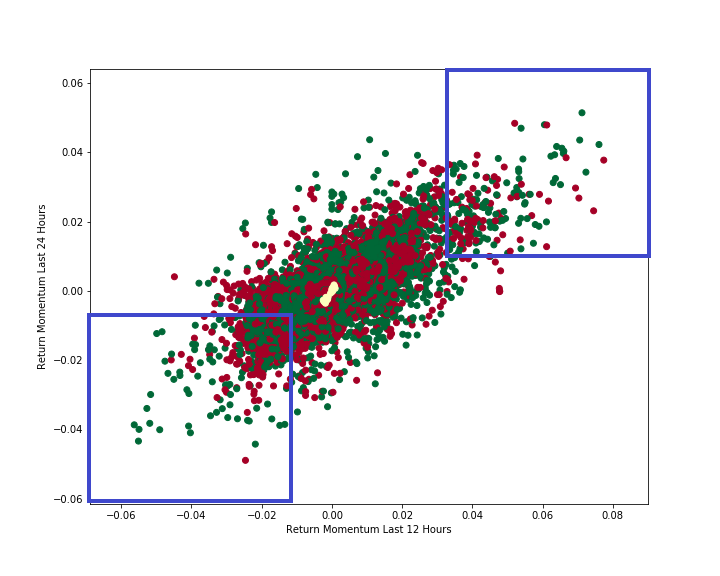
\includegraphics[width=0.5\textwidth]{EURUSDMomentum}
  %  below is only a naming convention, above is the real deal
    \label{fig:EURUSDMomentum}
     \caption*{Source: EURUSD FX Rate, Kaggle Database}
\end{figure}
Even in such a simple split of the predictor space, we see some evidence that more subsequent positive days occur in the bottom left of the chart (when prior 12 and 24 hour moves in the currency have been negative). Tree based methods use this type of inference to make predictions on future data points. The goal of the decision tree is to find multiple regions which then minimise the squared error of predictions
\begin{align}
\sum^{J}_{j = 1}\sum^{R_{j}}_{i = 1} (y_{i}-y^{*}_{R_{j}})^{2} 
\end{align}
 where $y^{*}_{R_{j}}$ is the mean response for the training observation within the $j^{th}$ region.
The methods tested in the project will revolve around Random Forests (introduced by Leo Breiman \cite{Breiman2001}) which averages the prediction across hundreds of single decision trees. 
\subsubsection{Background Research}
Research has shown that Random forests can generalise better than single decision trees as they maintain the high variance while reducing the bias of the model\cite{Genuer2012}.
 Random forests use bootstrapping to take multiple samples from the training data and also randomly samples the data and a subset of feature vectors to create a diverse array of decision trees to assist with the generalisation of the model. This method helps to create decision trees which are uncorrelated to each other and thus have lower probability of overfitting the data. Patel et al. showed that the it was possible to achieve classification rates of over 80\% for various stock price predictions when using the random forest algorithm and input features which consisted of technical price based indicators\cite{Patel2015}. The research used a random selection of three feature vectors (out of a total of ten) to create each single decision tree in the random forest model and tested the results from 20 to 200 trees using a majority vote for the final classification.  \newline
Kumar et al. performed extensive tests to compare the performance of support vector machines to random forests and found that on average support vector machines outperformed random forests when predicting the direction of the Indian stock exchange \cite{Kumar2006}. Three predictors were considered for each node while the number of trees for each model ranged from 200 to 1500, however there was no significant effect on the reduction of error rate for the out-of-sample data based on the number of trees. The RF model achieved classification rates of over 67\% on out of sample data.\newline
Chatzis et al. found that RF methods outperformed SVMs and logistic regression techniques when predicting stock market crisis events, they also note that RF models are relatively robust to overfitting due to each forest only being exposed to a subset of the available feature vectors \cite{Chatzis}.
The allure of using an ensemble method when using decision trees (DT) is that those models on an individual basis have low bias but high variance. However combining these models in an ensemble fashion can help to reduce the probability of overfitting, while improving model generalisation on unseen new data.
 

\section{Proposed Methodology}
The following section will outline the methodology to achieve the main projects aim and objectives that were outlined in section 2.
One area which looks to be under researched (in the view of the author) is a combination of models to handle different aspects of the trade signal generation process. This has the potential to perform well, as one model alone is unlikely to generalise into the future, especially when applied to the the domain of trading, where structural breaks can occur. \par Neural Networks, by the nature of their construction, need a large training set to understand the patterns within the data, thus this type of model could assist in the creation of higher frequency signals while a separate model can capture the market regime. \newline However, as we have mentioned previously, patterns in financial data remain exceedingly complex and the performance of one model could be due to a particular market regime. For example, regimes of strong investor risk appetite is an environment conducive to the positive performance of higher yielding currencies regardless of underlying country specific fundamentals \cite{Christiansen2011}. \newline Thus for a model to be successful, it must be capable of capturing changes in signal dynamics across different market regimes. This can be achieved by feeding features which also allow us to capture risk appetite, overall economic performance or mean reverting price patterns. 
\newline As pointed out by \cite{Mclean2016}, financial model performance can differ vastly prior to publication than after it \footnote{Research suggested a 26\% fall in performance out-of-sample and 58\% decline post publication}, whether due to over fitting or post publication anomaly decay \cite{Bartram2019}, this means we must be extra vigilante when assessing model performance.
\par The Python programming language (Python 3.6,\cite{McKinney1976}) will be used as the main programming application to achieve the objectives, with the python packages of Numpy \cite{VanDerWalt2011}, Scipy\cite{Tobergte2013}, Sci-Kit Learn\cite{Geron2017}, Matplotlib\cite{Wood2015} and Pandas\cite{Reiff2002} all providing very useful data manipulation functions to help store, clean and process data. For more complex ANN learning, the machine learning package Keras \cite{Chollet2015} will be used in the training and testing of ANN models.



\subsubsection{Objective 1: Data Capture, Cleaning and Standardisation}

The initial step will be to source intraday hourly price data for a selection of currencies\footnote{Analysis will involve developed market currencies of EUR, USD, JPY, GBP, SEK, NOK, AUD, NZD, CAD, CHF} and related economic and investor flow data. Figure \ref{fig:EURUSDPrice} shows the performance of EURUSD over the last sixteen years formed of hourly snapshots\footnote{circa 90,000 observations}
\newline There is evidence of the existence of momentum in currencies, and using higher frequency data can allow us to explore different time frames which have the most consistent momentum \cite{Filippou2017}. 
\begin{figure}[h]
    \centering
% below is where you put the acutal image name in the directory
	\caption{EURUSD Price Action}
    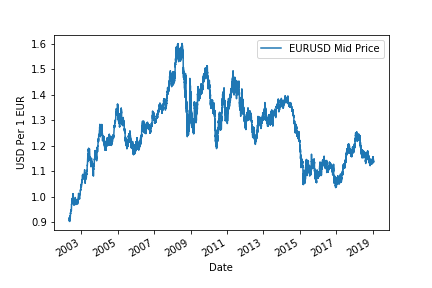
\includegraphics[width=0.5\textwidth]{EURUSDPrice}   
 %  below is only a naming convention, above is the real deal
    \label{fig:EURUSDPrice}
\caption*{Source: EURUSD FX Rate, Kaggle Database}
\end{figure}
Economic data can be obtained from a variety of sources, with the Federal Reserve Economic Database (FRED)\footnote{Successfully used in \cite{Chatzis2018} to assist with forecasting stock market crises}, IMF and OECD all providing vast treasures of low frequency economic data to create feature vectors. Relative economic growth (as measured by momentum across indicators such as consumer spending, GDP growth, industrial production and business confidence) has been shown to assist in the prediction of currency movements \cite{Dahlquist2015}.  
\newline The data will be stored and manipulated using Pandas dataframes while Sci-Kit Learn has some very useful functions such as StandardScaler which can standardise data using various different techniques (z-scoring, min-max etc).
\par Standarising the data remains an important initial step that has been used across a wide variety of prior research. Subtracting the mean and dividing by the standard deviation (z-scoring) \cite{Fischer2018}, min-max standardisation (\cite{Gunduz2017},\cite{Kumar2006})  and other techniques such as  mapping functions to scale feature vectors onto a pre-defined scale (\cite{Kara2011},\cite{Wang2014},\cite{Patel2015}) all help to achieve the overall goal of scaling, which is to ensure that larger or more volatile features do not overwhelm features of smaller magnitude and lower volatility. 
\newline Any errors or missing data will need to be rectified and as such the data will be tested for outliers which are impossible ( i.e. negative currency values) or do not fall within appropriate bands (.i.e 100\% percent jumps in currency values between hourly time frames). Cleaning of the data will be broken down into outlier detection (to capture any erroneous inputs) and cross checking the data vs known events in time (such as Brexit, election dates) to see if the observed outliers match the expected time frames. This provides some clarity on the time snapshot of the data as well. The time series will be transformed to a GMT date timescale so that there are no mis-matched values and to ensure the signal lags have been appropriately adhered to. 
\newline Sci-Kit Learn also provides functions to handle unbalanced datasets and anomaly detection which will be used to assit in cleaning the raw data \cite{anomalydetection} 


\subsubsection{Objective 2: Feature Selection} 
When working with financial time series the feature selection process should be driven by economic intuition as this can lessen the probability of over-fitting \cite{Arnott2018}. \newline As patterns and correlations in prices can change quite quickly, it is important not to over-fit the model on the data. A transformation of the data is also needed, with some findings suggesting that performing principal component analysis to create lower dimensional features as a robust method for creating predictive models \cite{Song2010}. The majority of previous research used price-based technical indicators \cite{Kara2011} \cite{Wang2014} \cite{Patel2015} \cite{Gunduz2017} such as moving average crossovers, rate of price change, average true range (ATR) and exponential moving averages to try to predict future currency direction. While technical indicators can be useful to forecast currencies, it is also important to measure non price based information such as economic momentum and valuation. The proposed feature set is outlined in table \ref{table:feature}.
\begin{table}[h] 
\centering      % used for centering table
\caption{Model Features} % title of Table 
\resizebox{\columnwidth}{!}{% 
\begin{tabular}{l l l}  % centered columns (3 columns) 
\hline                     %inserts double horizontal lines 
Indicator & Description &  Type \\ [0.5ex] % inserts table %heading
 \hline                    % inserts single horizontal line 
Short Term Momentum & 5,10, 21, 55 period Moving Average & Technical \\   % inserting body of the table
Long Term Momentum & 100, 155, 200, 255 Period Moving Average  & Technical \\ 
Mean Reversion  & Standard Deviation from 55, 100, 200 Period Moving Average & Technical\\ 
Volatility & 55, 100, 200 Period Rolling Volatility & Technical\\ 
Relative Economic Momentum & 1 Year Economic Momentum & Economic\\ 
Global Economic Momentum & 1 Year Global Economic Momentum & Economic\\
Purchasing Power Parity & Deviation From Fair Value & Fundamental Valuation \\[1ex]
\hline     %inserts single line 
\end{tabular} %
}
\label{table:feature} % is used to refer this table in the text 
\end{table} 

\subsubsection{Objective 3: Model Training and Fine Tuning}
The model training stage allows the learning algorithm to understand and capture the relationship between the features and the classification target vector (the target vector will be the future direction of the asset price across various time periods, both regression and classification models will be tested). Prior research has generally used binary classification of the future asset price move when developing models(\cite{Abreu2018},\cite{Gunduz2017}),\cite{Chatzis2018}). \newline Model training will also allow us to tune parameters to help to understand which combination of models (ANN, RNN, PNN ,SVM, RF) and underlying architecture (hidden layers, number of decision trees) are best suited in capturing the nuances in the data. This stage of the process will also allow experimentation with various  models to see the differences in performance. Various Python packages such as Sci-Kit Learn and Keras will be used in order to create and test the classification success rates of each type of model. Fischer et al. made use of Keras (on top of Googles Tensorflow) to implement Recurrent Neural Networks (RNN) \cite{Fischer2018} while using Sci-Kit Learn for logistic regression, SVM and Random Forest methods. \newline This is also a time where testing various combinations of models may work, one model may create a high frequency currency signal while a separate model identifies the regime where this model has historically performed the best. This stacked type of model architecture can assist in model generalisation and boost overall predictive performance (\cite{Chatzis2018},\cite{Stock2010}).


 
\subsubsection{Objective 4: Model Validation and Strategy Back testing}
In order to validate the model, the selected model and its structure will need to be tested in a similar setting to real world trading. This requires the construction of a backtesting engine which can simulate the models performance taking into account transaction costs and the funding costs associated with trading currencies.
This will provide a much more accurate analysis of the selected trading strategy performance. While classification success rates will be important in gauging model accuracy, high classification rates may not lead to positive strategy performance if large currency moves are mis-classified. Further analysis of model validation techniques are discussed in detail in the next section.


\subsection{Performance Evaluation}
Analysing and outlining model performance will be one of the key objectives to be satisfied in the final stages of the project.
In light of the findings from(\cite{Arnott2018},\cite{Bailey2013}), which highlight in detail the pitfalls inherent in systematic trading, the below outlines the approach to reviewing and evaluating model performance to standards generally set in financial institutions.


\subsubsection{Model Validation}
Once the model has been trained, then we begin the process of testing how the model performs on unseen data. This allows the model to score itself on previous iterations to understand the non-linear relationships within the data.
\subsubsection{Results Across All Model Iterations} 
Keeping track of the number of models being tested is very important as it can help define the statistical likelihood of finding a strategy that is a true positive. Even given 20 randomly selected strategies, there is a high probability that one strategy will beat the threshold needed for a statistical significance \cite{Arnott2018}. Thus, the number of trials ran must be considered so we can deflate the statistical significance of the strategy performance as a function of the number of trials\cite{Bailey2011}.
\subsubsection{Cross Validation}
Splitting the dataset into various training and test sets will be very important in being able to assess model performance. The most common cross validation techniques are K-fold cross validation and Leave-One-Out cross validation. This project will use a training set, validation set and finally a test dataset which will be held out until the final model has been selected. This will provide a useful gauge of out of sample performance\footnote{In depth study of cross validation techniques outlined in \cite{Bergmeir2012}}.
\subsubsection{Problem of Dimensionality}
 In finance, the lack of sufficient data (price) vs the number of possible predictors does lead to the issue of dimensionality, where we can add further features but not necessarily add further data points to be tested. Thus the model proposed here will remain cognizant of the number of features being used and will try to reduce the probability of finding false positive trading strategies. The dimensionality of the current data set will involve one target vector (i.e. future price move) and 17-20 predictor columns as outlined in \ref{table:feature}.
\subsubsection{Out-of-Sample Testing on Unseen Data}
 As stated by \cite{Arnott2018}, selection of model inputs is inherently biased (especially when done by domain experts) as the experts use heuristics to choose what they find the most economically intuitive as predictors, thus even out of sample test results are not fully out of sample. To override some of these concerns, this paper proposes to omit one years worth of data from any analysis until the model and related architecture has been fully completed and the selected model or average of model outcomes have been finalized. Then the chosen model will be blind tested on the final year of data that has been held back to give the best approximation of how the chosen model might have performed. 
\subsubsection{Simplicity Trumps Complexity}
The goal of this project is to try to create a model capable of generalising into the future, therefore it is important to choose an architecture which remain the simplest in terms of construction and feature sets. All models should be compared against a simple linear model as a benchmark, to test whether the value added by the increased complexity and reduced interpretability is substantial enough to over come the drawbacks. 

\subsection{Assessing Model Performance}

\subsubsection{Mean Squared Error}
The mean squared error (MSE) is used to measure the prediction accuracy of the model. It looks at the average distance of the predicted variable from the actual value .
\begin{align}
MSE = \frac{1}{N}\sum^{n}_{i = 1} (y_{i}-F(x_{i}))^{2} 
\end{align}
where $y_{i}$ is the actual value and $F(x_{i})$ is the value predicted by the function when the $i_{th}$ observation from is passed to the function. Generally speaking common practice would be to choose the model which has the lowest test MSE. \newline
\subsubsection{Precision and Recall}
Another method of model valuation is to look at the precision and recall of the model \cite{Patel2015}, whose values can be calculated from a confusion matrix, which shows the number of correct and incorrect classifications per class. Table \ref{table:confusion}  shows the confusion matrix for a two class classification problem.
\begin{table}[h] 
\centering      % used for centering table 
\caption{Confusion Matrix} % title of Table 
\resizebox{.75\textwidth}{!}{%

\begin{tabular}{l l l}  % centered columns (3 columns) 
\hline                     %inserts double horizontal lines 
Actual (row) Predicted (col) & Buy &  Sell \\ [0.5ex] % inserts table %heading
 \hline                    % inserts single horizontal line 
Buy & True Positive & False Negative \\   % inserting body of the table
Sell & False Positive & True Negative \\ [1ex]
\hline     %inserts single line 
\end{tabular} %
}
\label{table:confusion} % is used to refer this table in the text 
\end{table} 

The confusion matrix allows us to calculate the precision and recall of the model, the formulas for which are shown below.
\begin{align}
Precision = \frac{True Positive}{True Positive + False Positive} 
\end{align}
\begin{align}
Recall = \frac{True Positive}{True Positive + False Negatives} 
\end{align}
The precision tells us how well the model has performed in terms of the number of positive signals (correct buy signals as a percentage of all buy signals) that were actually triggered,while recall of the model depicts how accurate the model has been as a function of the total number of positives in the data set itself. This is an important metric to analyze when predicting a financial time series as certain periods can be heavily biased towards one class or another, for example in the case of a financial asset which has a strong trend will by design have a higher occurrence of one class vs another.


\subsubsection{Deflated Sharpe Ratio}
Given the inherent issues of overfitting in Finance (\cite{Arnott2018},\cite{LopezdePrado2018}), it is also important to analyse the overall Sharpe Ratio \cite{Sharpe2009} which measures the overall return of a trading model relative to its risk (or volatility of returns). \newline High Sharpe ratios can be obtained by a genuinely good model or through pure overfitting/selection bias, thus it is important to deflate the Sharpe Ratio of every strategy tested to take into account the number of models tests as well as the skew of each strategies distribution \cite{Bailey2014}. 
The Deflated Sharpe Ratio is a test statistic which can outline the probability of having found a true positive. It is defined below as
\begin{align}
\widehat{DSR} = \left[
		 				\frac{\widehat{SR}-\widehat{SR_{0}}\sqrt{T-1}}
						{\sqrt{1-\gamma_{3}\widehat{SR} + \frac{\gamma_{4} - 1}{4}*\widehat{SR}^{2}}} 
				 \right]
\end{align}
where $\widehat{SR} = \sqrt{V\left[\widehat{SR}_{n}\right] 
						\left(      	
							\left(1- \gamma\right) Z^{-1} \left[ 1- \frac{1}{N}\right] + \gamma Z^{}-1 \left[ 1-\frac{1}{N}\exp^(-1) \right] 
						 \right)}$
and $\widehat{SR}$ is the estimated Sharpe Ratio, $T$ is the sample length, $\gamma_{3}$ is the skewness of the returns distribution and $\gamma_{4}$ is the kurtotis of the selected strategy,  $V\left[\widehat{SR}_{n}\right]$ is the variance across the number of strategy Sharpe Ratios tested, $N$ is the number of independent trials of strategies run (.i.e. the number of models tested) and $Z$ is the cumulative function of the Gaussian distribution\footnote{Further information and theoretical proofs of the Deflated Sharpe is available from \cite{Bailey2014}}.  

\section{Proposed Work plan}
The next page will outline the necessary steps to undertake the work needed. In total, this will require just over 300 hours of work, from the end of April until the deadline date in September 2019.

\begin{sidewaystable}[h] \caption{Proposed Work Plan} % title of Table 
\centering      % used for centering table 
\begin{tabular}{c | c c c c}  % centered columns (4 columns) 
\hline                     %inserts double horizontal lines 
Objective         & Task                &   Description                                                                               & Start Date          & Completion Date \\ [0.5ex] % inserts table %heading
 \hline                    % inserts single horizontal line 
   		   & Data Retrieval        & Source data from various public and institutional databases     & April 20$^{th}$   & April 26$^{th}$\\   % inserting body of the table
1 & Data Cleaning         & Screen data for outliers                                                         & April 27$^{th}$    & May 5$^{th}$ \\ 
    		    & Truncation              & Split data into appropriate training and testing sets                 & May5$^{th}$      & May6$^{th}$ \\ 
   		   & Standardization        & Transform and Center data                                                    & May$6^{th}$       & May 7$^{th}$ \\
\hline
   		  & Choose Target        & Choose variable to be classified                                              & May 8$^{th}$ & May 9$^{th}$\\ 
2  		& Feature Selection    & Select intuitive features for the model                                    & June$14^{th}$ & June 30$^{th}$\\ 
    		& Model Preprocessing & Choose the features appropriate for each model                    & July$1^{st}$ & July 3$^{rd}$\\
\hline
   		& Architecture Selection & Analyse various model combinations                                  & July$12^{th}$ & July 28$^{th}$ \\
  3  		& Model Training             & Run Various Training Iterations                                         & July$12^{th}$ & July 28$^{th}$ \\
		& Model Tuning               & Run Various Model Architectures                                       & July$12^{th}$ & July 28$^{th}$ \\
\hline    
    		& Model Validation           & Cross Validation Across Models                                         & July$28^{th}$ & August 10$^{th}$ \\
 4  		& Backtesting                  & Run trading signals through backtester engine                   & August$12^{th}$ & August 20$^{th}$ \\
     		& Bench-marking            & Compare final model to linear/trivial classifier                    & August$21^{st}$ & August 25$^{th}$ \\
\hline
 	    	& Blind Testing                & Run finalised model on Blind data                                    & August$26^{th}$ & August 26$^{th}$\\
5       	& Performance Evaluation & Analyse Performance Statistics                                       & August$27^{th}$ & September 3$^{rd}$\\        % [1ex] adds vertical space 
		& Final Project Report       & Collate Results and Findings                        		       & August$27^{th}$ & September 3$^{rd}$\\  [1ex]
\hline     %inserts single line 
\end{tabular} \label{table:nonlin}  % is used to refer this table in the text 
\end{sidewaystable} 
\clearpage

\subsection{Time Allocation and Potential Risks}
Table \ref{table:nonlin} provides a guideline towards the time allocated to each task, the chronological order of the task may change as more the further into the work develops it may be necessary to go back and add more features or implement the model architecture differently. Some risks to the timeline of events are listed below.

\subsubsection{Data Consistency}
Going forward, there could be data access issues or that the data does not exist in a consistent format or that the database where the data was previously available is removed of public use. The solution to this would be to search for new databases with similar information or to continue ahead with data already retrieved.
\subsubsection{Poor Feature Selection}
By the stage of model training, it may become evident that the original features selected have little predictive power, to solve this, new data sources could be utilised or innovative transformations made on the existing data so that new avenues of relationships between the predictors and dependent variables are uncovered.

\subsubsection{Under Allocation of Resources}
It may become evident over the course of the project that too little computing resources have been allocated to train the models, this may require the use of cloud based GPUs \footnote{Available from Google Cloud or Amazon Web Services} to speed up learning and the production of meaningful results. 
\subsubsection{Look Ahead Bias}
Performance of the results will be skewed by any errors in the data selection or model training process, one common pitfall to avoid is that the features are not using data that would not have been available at the initial time of classification such that the model is using future data.


\bibliography{ref_list}{}
\bibliographystyle{ieeetr} % could also use apalike, ieeetr , abbrv
%\printbibliography
% this moves us to a new page...
\clearpage


\end{document}